\chapter{Cryptographic Primitives}

\section{Hash Functions}\index{Hash Function}

We already discussed the \emph{gossip protocol} that allows peer-to-peer nodes to exchange
objects on the network. Before exchanging an object, it is useful that the nodes can talk
\emph{about} these objects and ask each other whether they have a particular object. To
do this, it will be useful to give each object a unique identifier. We cannot use
increasing integers as identifiers, as these objects may be created in different parts of
the network and there is no global shared counter. We also cannot use a simple random
number as the identifier, as we want the identifier to be unfakeable: Given an identifier
we want to be able to check that the object really does correspond to the identifier.

For this, we will use \emph{cryptographically secure hash functions}\index{Hash function}. The hash function
is a function
\glsxtrnewsymbol[description={hash function}]{hash}{$H$}\glsadd{hash}
$H: \{0, 1\}^* \longrightarrow \{0, 1\}^\kappa$,
where $\kappa$ is the
security parameter. As you can see, the hash function accepts \emph{any} string as input,
but \emph{always} returns a $\kappa$ bits long string. This makes it useful as a
\emph{compression} mechanism, as these identifiers are short ($\kappa$ will be $256$
bits in practice) and can be exchanged on the network prior to the actual objects. In order for $H$ to be practically useful, we require that it is polynomially computable.

\subsection*{Collision Resistance}

Ideally, we would like each different object to correspond to exactly one hash
output:

\[
  \forall x_1, x_2: x_1 \neq x_2 \Rightarrow H(x_1) \neq H(x_1)
\]

However, this ideal goal is unattainable.
Because the hash function has \emph{unlimited} inputs and \emph{limited} outputs,
there will necessarily exist some \emph{collision} in which multiple inputs correspond
to the same output. To find a collision, we can start enumerating all the possible
inputs to the hash function starting at $0$ and going up to $2^\kappa$. If we have
not found a collision when we reach $2^\kappa - 1$, then this means that we have taken
up all of the possible $2^\kappa$ outputs. When we then evaluate the hash function on
the input $2^\kappa$, we will certainly find a collision. This process is shown in
Algorithm~\ref{alg.hash-collision}.

\import{./}{algorithms/alg.hash-collision}

Of course, as this function has to run through
$2^{2\kappa}$ combinations, its running time is exponential. The result that hash
functions must \emph{necessarily} have collisions stems from the Pigeonhole
Principle~\cite{liu}:

\begin{theorem}[Pigeonhole]\index{Pigeonhole Principle}
  Consider a function $f: A \longrightarrow B$. If $|A| > |B|$, then there must
  exist $x_1$ and $x_2$ such that $f(x_1) = f(x_2)$.
\end{theorem}

Instead, we will require that \emph{finding} such collisions is \emph{computationally}
difficult. We can define this in the form of the collision finding cryptographic game,
illustrated in Algorithm~\ref{alg.collision-game}.\index{Collision Resistance}

\import{./}{algorithms/alg.collision-game}

In this game, we ask the adversary to produce two different inputs $x_1$ and $x_2$
that have the same hash. Note that the hash function $H$ is different
for every value of $\kappa$ (while the code that produces the hash output for every
$\kappa$ is the same, it must take $\kappa$ into account when running), so we
denote it $H_\kappa$. It gives $\kappa$ bits of output. The adversary can have some
hard-coded collisions in her source code, but, if our hash function is secure, these won't
work\footnote{If you come from the field of cryptography,
note that here we're bypassing the gory details of \emph{keyed} hash functions
by requiring the adversary be uniform.}
for sufficiently large values of $\kappa$.

\subsection*{Gossiping with Hashes}

Collision resistance ensures that, if we are given a hash of something, we cannot
later be given something else that hashes to the same value. Each object's hash
is uniquely identified by its content. We say that objects are
\emph{content addressable}\index{Content Addressable}
by their hashes.
This makes hashes suitable
for use as identifiers of objects as we exchange them on the network. When gossiping
about objects, instead of sending a whole object to each of our peers, we can optimize
the process by advertising the ownership of an object through its hash. The hash of
an object used in this manner is called the \emph{objectid}. If the peer already knows
about this object, they can ignore our advertisement. If the peer has not seen the
object before, they can request the object through its objectid. Only at this point, we
send the full object to the peer. Upon receiving the object, the peer can verify that
it is indeed the requested object by hashing it and comparing it to the stored objectid.
Towards this purpose, each node must maintain a set of known objectids for quick lookup.

We now have a more complete understanding of how the gossiping protocol works,
illustrated in Figure~\ref{fig:gossiping-via-hashing}:

\begin{enumerate}
  \item Node $A$ first becomes aware of a new object $O$, either by receiving it from a peer,
        or by generating it locally. Object $O$ has objectid $h = H(O)$, where the input to the
        hash function is a string-encoded version of the object.
  \item $A$ advertises its knowledge of $O$ by sending a message
        indicating \emph{I have an object with objectid} $h$ to its peer $B$.
  \item $B$ receives the objectid $h$ and checks against its database whether it has already seen
        this object. Suppose that it has not. At this point, $B$ sends to $A$ a message
        requesting the contents of the object with objectid $h$.
  \item $A$ sends to $B$ the object $O$. Upon receiving $O$, the node $B$ can verify that
        $h = H(O)$, where $h$ is the requested objectid. This ensures that $A$ sent the
        correct object to $B$.
  \item In turn, $B$ advertises to \emph{its} peers that it now knows of an object with
        objectid $h$. It sends node $C$ a message indicating this.
  \item At this point, if $C$ has already received $O$ from $A$, it will not request
        the object from $B$. This is how the propagation in the gossiping algorithm stops.
\end{enumerate}

\begin{figure}
    \centering
    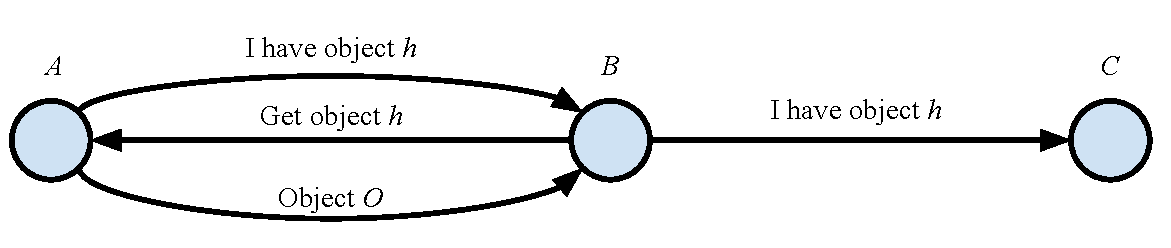
\includegraphics[width=\columnwidth,keepaspectratio]{figures/gossiping-via-hashing.pdf}
    \caption{Gossiping via hashing. The hash function $H$ is used to give content-addressible hash $h$ to object $O$.}
    \label{fig:gossiping-via-hashing}
\end{figure}

The node $B$ does not know whether $h$ was newly generated by $A$, or if $A$ is simply relaying.
This gives a modicum of anonymity: When a new object is first sent to us from an IP address,
we cannot deduce that the message is actually originating from that IP address.

\subsection*{Preimage resistance}

Hashes are also useful for allowing a party to \emph{commit} to a value. The party
reveals that hash, but not the object itself. Anyone who has the hash can verify that
the object is correct once the full object has been received, but it is useful that
this is not possible when seeing only the hash: It should be difficult to find the
\emph{preimage} of a hash given its image. Of course, the preimage of a hash can
be found by performing an exhaustive search in a similar fashion to
Algorithm~\ref{alg.hash-collision}, but this will take exponential time.
Naturally, we can define the property of \emph{preimage resistance} using a
cryptographic game.\index{Preimage Resistance}

\import{./}{algorithms/alg.preimage-game}

In this game, the challenger chooses a random $\kappa$-bit value as the input. This is denoted by
the $x \getsrandomly S$ symbol that indicates that an element $x$ is chosen uniformly at random
from the set $S$. Note here that to do this, the challenger, too, has access to randomness,
and so any probabilities are also taken with respect to this randomness.
The adversary is given $H(x)$ and would like to find $x$.
As there are other inputs that produce the same $H(x)$,
we ask her to produce some $x'$ (equal or different from $x$) that has the same hash value
as $x$.

But, perhaps, we are simply asking too much of this adversary. It would already be a big problem
for us if the adversary, given some $x_1$, can find a \emph{different} $x_2$ that hashes to the same
value. We call this property \emph{second primage resistance}, and it is defined through the following
game.\index{2nd Preimage Resistance}

\import{./}{algorithms/alg.2preimage-game}

In this game, the adversary is given a randomly sampled $(2\kappa+1)$-bit string input $x_1$ by the challenger .
The adversary is successful if she can come up with an $x_2 \neq x_1$ that hashes to the same value as $x_1$

It seems that all three properties, collision resistance, preimage resistance, and second preimage
resistance, are desirable. Let us examine whether some of these properties are stronger than the other.
Finding a collision seems to be the easiest: The adversary is asked to come up with her own $x_1, x_2$,
without any input from the challenger. The preimage adversaries seem stronger: If we have
an adversary who can produce a preimage, we can use her to create a collision. Collisions require
that $x_1 \neq x_2$. We now show that preimage resistance implies collision resistance.

\begin{theorem}[Collision Resistance $\implies$ Preimage Resistance]
  \label{thm.collision-2preimage}
  If a hash function $H$ is collision resistant, then it is 2nd preimage resistant.
\end{theorem}
\begin{proof}
  Suppose, towards a contradiction, that $H$ is collision resistant but not 2nd preimage resistant.
  Then, there exists an adversary $\mathcal{A}$ that can win the 2nd preimage game with non-negligible probability $Pr_\mathcal{A}$. We will construct an adversary $\mathcal{A}'$ against the
  collision challenger which uses $\mathcal{A}$ as a black box.

  The adversary $\mathcal{A}'$ works as illustrated in Algorithm~\ref{alg.collision-2preimage}. She first chooses an $x_1$ uniformly at random from the message space. She then hands this $x_1$ to $\mathcal{A}$, who, hopefully, produces an $x_2$ such that $x_1 \neq x_2$ and $H(x_1) \neq H(x_2)$. The adversary $\mathcal{A}'$ outputs the pair $(x_1, x_2)$.

  If the adversary $\mathcal{A}$ is successful in breaking the 2nd preimage game, then $\mathcal{A}'$ will be successful in breaking the collision game:

  \[
    \Pr[\textsf{preimage-game}_\mathcal{A}(\kappa)]
    =
    \Pr[\textsf{collision-game}_{\mathcal{A}'}(\kappa)]
  \]

  Since $\Pr[\textsf{preimage-game}_\mathcal{A}(\kappa)]$ is non-negligible, then so is $\Pr[\textsf{collision-game}_{\mathcal{A}'}(\kappa)]$.

  Furthermore, the adversary $\mathcal{A}'$ works in polynomial time, and so is also PPT. This contradicts the assumption that $H$ is collision resistant.
\end{proof}

% TODO: Redraw and improve this figure (in PDF format)
\begin{figure}[H]
    \centering
    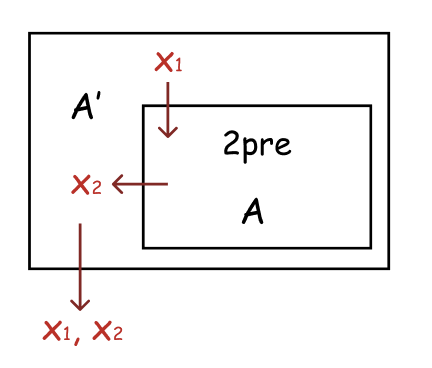
\includegraphics[scale=0.6]{figures/2pre.png}
    \caption{A visualization of Theorem~\ref{thm.collision-2preimage}.}
    \label{fig:2pre_viz}
\end{figure}

\import{./}{algorithms/alg.collision-2preimage}

In addition, an adversary who breaks preimage resistant is stronger than an adversary who breaks 2nd preimage resistant. This is not surprising. An adversary who works towards finding a second preimage already has a first preimage, whereas an adversary who attempts to break preimage resistance only has an image.

This is captured in the following theorem:

\begin{theorem}[2nd Preimage Resistance $\implies$ Preimage Resistance]
  \label{thm.2preimage-preimage}
  If a hash function $H$ is 2nd preimage resistant, then it is preimage resistant.
\end{theorem}
\begin{proof}
  Consider a PPT adversary $\mathcal{A}$ against the preimage game.
  We will construct an adversary $\mathcal{A}'$ against the 2nd preimage game. The adversary $\mathcal{A}'$ is depicted
  in Algorithm~\ref{alg.2preimage-preimage}. It is clear that $\mathcal{A}'$ is PPT because $\mathcal{A}$ is PPT.

  \import{./}{algorithms/alg.2preimage-preimage}

  Even though $\mathcal{A}$ could win the preimage game, this only guarantees that $H(x_1) = H(x_2)$.
  We need one additional property for $\mathcal{A}'$ to win the 2nd preimage game: It must hold that $x_1 \neq x_2$.
  We will now argue that this is often the case.

  To do this, we draw the input space as a big box with
  each input illustrated as a pink dot, as shown in Figure~\ref{fig.2preimage-preimage}. There are $2^{2\kappa + 1}$ dots in the big box. We now partition this big box into smaller boxes, grouping each input with the other inputs that have the same image. We move the larger boxes (containing more dots) to the left of the picture and the smaller boxes (containing fewer dots) to the right of the picture.

  \begin{figure}[H]
    \centering
    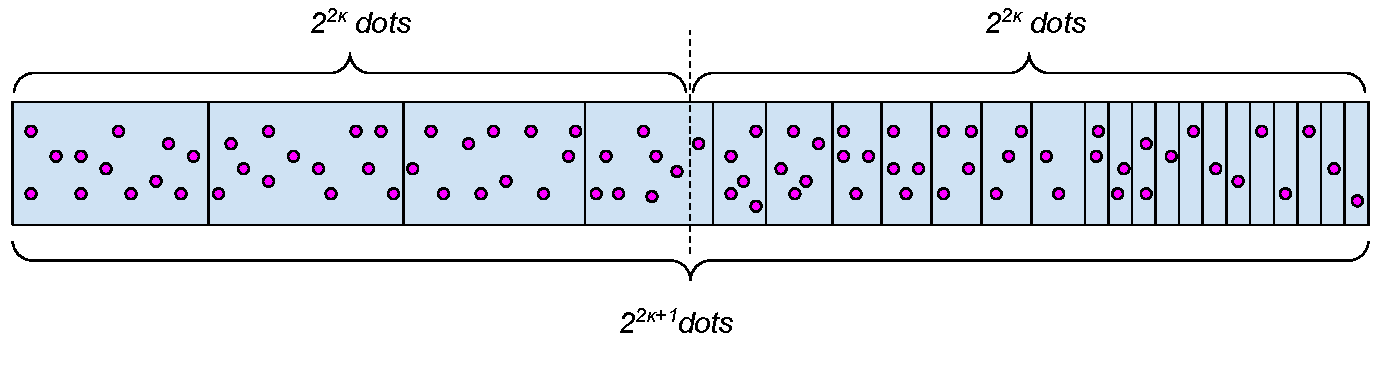
\includegraphics[width=\columnwidth,keepaspectratio]{figures/2preimage-preimage.pdf}
    \caption{A visualization of Theorem~\ref{thm.collision-2preimage}.}
    \label{fig.2preimage-preimage}
  \end{figure}

  We now split the big box into two big partitions exactly in the middle, as illustrated by the vertical dashed line, with $2^{2\kappa}$ dots on the left, and $2^{2\kappa}$ dots on the right (the dashed line may cut one of the smaller boxes in the middle, but this is fine).

  We now argue that the boxes on the left of the dashed line are large.

  \textbf{Claim: } \emph{Each of the boxes to the left of, or on, the dashed line contains at least $2^\kappa$ dots.} To see this, we need a counting argument. Towards a contradiction, suppose that one of the boxes to the left of, or on, the dashed line contains fewer than $2^\kappa$ dots. Then, since the boxes are ordered, each box on the right of the dashed line contains fewer than $2^\kappa$ dots. However, because the output space is only $2^\kappa$, this means that there are at most $2^\kappa$ boxes to the right of the dashed line. This means that, on the right of the dashed line, there can only be fewer than $2^\kappa$ dots $\times 2^\kappa$ boxes = $2^{2\kappa}$ dots. But there are exactly $2^{2\kappa}$ dots to the right of the dashed line by construction. Therefore the claim is true.

  Now that we have proven this claim, we can compare the probabilities of success of $\mathcal{A}$ and $\mathcal{A}'$. We will only consider the case where the uniform sampling of $x_1$ by the 2nd preimage challenger falls to the left of the dashed line. This happens with probability $\frac{1}{2}$. If this is the case, then there are at least $2^{\kappa}$ dots in the box of $H(x_1)$.

  Therefore, \emph{conditioned} on the fact that $\mathcal{A}$ is successful and that we have landed to the left of the dashed line, the probability of success of $\mathcal{A}'$ is $1 - 2^{\kappa}$. The overall probability of success of $\mathcal{A}'$ is

  \[
    \Pr[\textsf{2nd-preimage-game}_{\mathcal{A}'}(\kappa)] \geq \frac{1}{2} (1 - 2^{-\kappa}) \Pr[\textsf{preimage-game}_\mathcal{A}(\kappa)]\,.
  \]

  Since $H$ is 2nd preimage resistant, the probability $\Pr[\textsf{2nd-preimage-game}_{\mathcal{A}'}(\kappa)]$ is negligible.
  Then so is $\Pr[\textsf{preimage-game}_\mathcal{A}(\kappa)]$, because $\frac{1}{2}$ is a constant and $(1 - 2^{-\kappa})$ is a value larger than $\frac{1}{2}$. Therefore, $H$ is also preimage resistant.
\end{proof}

Note that in the above proof, the probabilities of success of $\mathcal{A}'$
and $\mathcal{A}$ are related by an inequality. This is because $\mathcal{A}'$
may also succeed in case we land to the right of the dashed line, but we are not
accounting for this probability in our counting.

Additionally, observe how we went in the \emph{forward direction} in this proof:
Contrary to previous proofs, we did not assume that $\mathcal{A}$ succeeds with non-negligible
probability at any point in the proof. As we have discussed in the previous chapter,
this is a cleaner way of writing security proofs, although it takes some getting used to.

\subsection*{Hash Security}

We can now define what it means for a hash function to be \emph{cryptographically secure}
or simply \emph{secure}. Since collision adversaries are the weakest adversaries, we will
simply require that our hash functions are collision resistant.

\begin{definition}[Secure Hash Function]
  A hash function $H: \{0, 1\}^* \longrightarrow \{0, 1\}^\kappa$ is \emph{secure} if there is a negligible function \emph{negl} such that

  \begin{gather*}
    \forall PPT \mathcal{A}:
      \Pr[\textsf{collision-game}_{H,\mathcal{A}}(\kappa)] = 1] \leq \textsf{negl}
  \end{gather*}
\end{definition}

\subsection*{Applied Hashes}

In practice, the hash functions most commonly used to build blockchains are
\texttt{SHA256} (used by Bitcoin), \texttt{SHA3} or \texttt{keccak} (used by Ethereum),
\texttt{blake2}, or Poseidon. As an example, \texttt{SHA256} is a hash function that takes
any input and outputs $\kappa = 256$ bits (or $32$ bytes). Here is the \texttt{SHA256} hash
of the word ``hello'', displayed in hexadecimal format:

\texttt{2cf24dba5fb0a30e26e83b2ac5b9e29e1b161e5c1fa7425e73043362938b9824}

% \section{Transactions and Signatures}
% \textbf{Verifiability of money}: If money is created correctly, money has verifiability property such as ownership validation. Here, we discuss a transfer of ownership.
%
% In blockchain networks, a transaction is an entry in local state. Each node keeps a ledger, which is a recorded sequence of transactions ("tx"s). Ledgers are used to verify and update the system state, a record of the balances of all parties in the system, such that consensus across nodes is maintained.
%
% Assume we have parties $A$, $B$, $C$, etc. Each party can have some sort of money and each party will share all financial information. An example of a transaction could be party $A$ saying "Give 5 units to party $B$." The following is an outline of ledger/transaction procedures:
% \begin{enumerate}
%     \item
%     Initial system state: some distribution of money.
%     \item
%     Issue a tx by broadcasting
%     \item
%     Upon receiving a tx:
%     \begin{enumerate}
%         \item
%         Check validity (source has enough money)
%         \item
%         Append to local ledger
%     \end{enumerate}
%     \item
%     Read ledger to determine balances (system state)
% \end{enumerate}
%
\section{Signatures}\index{Signature}

When Alice sends money to Bob, she needs to \emph{authorize} this payment. This means
that the rest of the network needs Bob to \emph{prove} that Alice really gave him
her money instead of taking his word for it.

We will use a cryptographic \emph{signature scheme} to do that. A cryptographic signature
scheme is a means for a party to say ``this message was really written by me'' and it is
not a forgery.

\subsection*{Public Key Cryptography}

Before we discuss signature schemes, we must discuss the notion of identity in the cryptographic
setting. In a traditional legal system, an identity is tied to a person's physical body
and authorized by a government using papers such as a passport. In our case, we do not want
to rely on physical bodies or centralized governments for proving identity. Anyone should be
able to create a new identity \emph{pseudonymously}\index{Identity}\index{Pseudonymity}, without necessarily associating it with
their real person. To do this, a participant uses his computer to create a \emph{key pair}.
The key pair consists of two keys: A \emph{public key}\index{Public key} and a \emph{secret key}\index{Secret Key}
(or \emph{private key}\index{Private Key}). The public key portion of the key pair can be shared freely and even
be made public. For example, it can be published on the owner's website, social media, or on
a newspaper, without any security problems. On the contrary, a private key must be kept secret.
We use the public key to specify \emph{the identity about which we are speaking}. So, instead
of saying ``Alice'' with such and such legal name, we refer to her by her public
key. The private key can be used by Alice herself to prove her identity. That's why the
private key must remain secret: If it falls into the hand of someone else, this someone
else \emph{really is} Alice. Of course, any physical person can create multiple different
key pairs and maintain multiple identities that are not necessarily associated with one
another. This idea will play an important role in achieving a basic level of pseudonymity.

The public key and private key are created together as a pair, because they are associated
with one another mathematically in a unique manner. For every private key, there is a unique
associated public key. For every public key, there is a unique associated private key.
Given a private key, it is \emph{easy} to get the respective public key. Given a public
key, it is \emph{hard} to get the respective private key, even though there is a unique
such key. This is essential. If it were easy to get the private key from a public key,
anyone who knew your public key could impersonate you. We will denote the public key
\glsxtrnewsymbol[description={public key}]{pubkey}{$pk$}\glsadd{pubkey}
$pk$
and the secret (or private) key
\glsxtrnewsymbol[description={secret key}]{seckey}{$sk$}\glsadd{seckey}
$sk$.

\subsection*{Unforgeability}

A cryptographic signature is created using a particular private key $sk$ and is
denoted
\glsxtrnewsymbol[description={signature}]{signature}{$\sigma$}\glsadd{signature}
$\sigma$.
It is associated with a particular message $m$. This means that
the person who holds the private key has authorized this message $m$. The message
will say something like: ``I, Alice, gave 5 monetary units to Bob.'' Of course, the
messages will be in a computer-readable format. We will make these messages more
precise very soon.

A signature is associated with a particular message. If the user wants to sign a
different message, a different signature must be created. If $\sigma$ is the signature
pertaining to the message $m$, then a signature $\sigma'$ must be created for a
different message $m' \neq m$. The signature $\sigma$ will be invalid for message $m'$.
This shows that cryptographic signatures are very different from hand-written signatures.
Hand-written signatures are useless from a security point of view, as they can be
copied and pasted around and their veracity cannot be checked. Cryptographic
signatures cannot be copied underneath unauthorized messages. This would constitute
a \emph{forgery}, and we will make a precise computer science claim about how
likely such forgeries are using a cryptographic game. We emphasize that we use the
word \emph{signature} because there is some analogy in physical signatures, but
what we are achieving here is something truly different and much more powerful
than pen-and-paper signatures. There is no reliance on courts of law and pseudoscientific
``graphologists'' to tell whether a signature is genuine. Instead, the reliance is
on hard computational problems and formal cryptographic claims.

Before we define our security game, let us precisely state how a signature protocol
works. Initially, Alice generates her key pair $(pk, sk)$ by invoking a special algorithm
$Gen(1^\kappa)$. The public key and the secret key are both simple strings, $\kappa$
bits long (in practice typically $256$ bits each).
She keeps $sk$ secret and publishes $pk$ by
sending it to her friends. When the time comes for Alice to write a message $m$
that she wishes to sign, she uses her private key $sk$ to invoke the function
\glsxtrnewsymbol[description={signature function}]{sig}{$Sig$}\glsadd{sig}
$Sig(sk, m)$
to obtain a signature $\sigma$. She sends the message $m$ together
with the signature $\sigma$ to Bob. Bob already holds the public key $pk$ of Alice.
He uses the public key to invoke the function
\glsxtrnewsymbol[description={signature verification}]{ver}{$Ver$}\glsadd{ver}
$Ver(pk, m, \sigma)$,
which returns
$\true$ if the signature was genuinely created by Alice, or $\false$ otherwise.
If the adversary sends a different message $m' \neq m$ together with this $\sigma$
to Bob, the \emph{Ver} function will return $\false$.

If both the sender and the verifier are honest, the signature scheme should always
work. This is what constitutes a \emph{correct} signature scheme.

\begin{definition}[Signature Correctness]
  Consider a signature scheme $(Gen, Sig, Ver)$. The scheme is \emph{correct} if
  for any key pair $(pk, sk)$ generated by invoking $Gen$, and
  for all messages $m$, it holds that $Ver(pk, m, Sig(sk, m)) = \true$.
\end{definition}

For the security definition, we want the adversary to not be able to produce
messages that were not authorized by their rightful owner. Since we are protecting
an honest verifier who holds a correctly generated public key, our challenger will
invoke \emph{Gen} to obtain the key pair $(pk, sk)$. Additionally, the adversary will
be given access to $pk$, since this is public, but not access to $sk$ (if the adversary
has access to $sk$, we can have no hope). The adversary will then attempt to generate
a signature $\sigma$ that verifies for a message $m$ using the public key $pk$.
The adversary does not have to use the \emph{Sig} algorithm, but can use any method
she likes, as long as the $Ver$ algorithm returns $\true$. The game will output
$\true$ if the $Ver$ algorithm outputs $\true$.

But note that this approach misses something: The adversary is trying to generate
signatures \emph{in the blind}, but in the real world, the adversary may see some
authorized signatures that the honest signer really \emph{did} make. The adversary
can then make use of these signatures as she sees fit. For example, she might try
to copy/paste a signature on a different message, or alter an existing signature
on one message to create a signature on a different message. We would like our
game to capture the fact that the adversary has this kind of access. To make her
even more powerful, in our game we allow the adversary to ask the signer to sign
\emph{any message of her choice}. As long as the adversary can produce a signature
for \emph{any message she did not ask a signature for}, we consider it a successful
forgery. This is a very powerful notion. The adversary has a lot of power, so if
we can create a signature scheme that is resilient to such adversaries, we will have
a lot of confidence in our protocol.

\import{./}{algorithms/alg.existential-forgery}

The \emph{existential forgery game} is depicted in Algorithm~\ref{alg.existential-forgery}.
Initially, the challenger generates a keypair $(pk, sk)$ using the honest key generation
algorithm \emph{Gen}. He then invokes the adversary, giving her access to $pk$. Since
$pk$ is $\kappa$ bits long, we do not need to pass $1^\kappa$ to this adversary.
A closure function $\mathcal{O}$ is defined within the challenger. When invoked
with a message $m$, this function gives out a signature $\sigma$ to the message
$m$ using the secret key $sk$, but without revealing the secret key. The closure
also records the requested message in the set $M$.
When the adversary is invoked, she is given \emph{oracle access} to call the
function $\mathcal{O}$. This is like a callback, and is denoted using the
exponent notation. It means that $\mathcal{A}$ can call $\mathcal{O}$, but
cannot look at its code. Critically, $\mathcal{A}$ cannot see the value $sk$.
The adversary can make multiple \emph{queries} to the oracle to obtain many
signatures. Based on the signatures she sees, she can make yet further queries
in an adaptive manner. When she is finally ready, the adversary is expected
to produce a signature $\sigma$ on a message $m$ that was not queried to the
oracle $\mathcal{O}$ (the adversary can trivially succeed in providing a signature
for messages queried to the oracle). If the message and signature provided by
the adversary pass the \emph{Ver} check using the public key $pk$, the adversary
is deemed successful.

The security definition is straightforward. Since we have already seen a few
identical security definitions, try writing out the definition before looking
at it.

\begin{definition}[Secure Signature Schemes]
  A signature scheme $(Gen, Sig, Ver)$ is called \emph{secure} if there
  exists a negligible function \emph{negl} such that

  \begin{align*}
    \forall PPT \mathcal{A}:
    \Pr[\textsf{existential-forgery}_{Gen, Sig, Ver, \mathcal{A}}(\kappa) = 1] < \textsf{negl}(\kappa)
  \end{align*}
\end{definition}

Secure signature schemes are sometimes called \emph{existentially unforgeable signature
schemes}\index{Existential Unforgeability}.

\subsection*{Applied Signatures}

Since the hash of a message is a unique identifier for it, it is sufficient that
the hash of a message is signed instead of the message itself. This is often done
in practice since it simplifies the implementation of signature schemes.
One class of secure signature schemes is called
\texttt{ECDSA}\index{ECDSA} and is based on the mathematical structure of \emph{elliptic curves}\index{Elliptic Curve}.
These curves define how public keys are structured, and they involve some algebra
which makes it hard for private keys to be calculated based on the knowledge of
just the public key. The computational problem on which hardness is based is called
the \emph{discrete logarithm problem}\index{Discrete Logarithm Problem}.
There are different curves with different names, and each of them
defines a different format for key pairs.
A popular curve in cryptocurrencies is
\texttt{secp256k1}\index{secp256k1}. Another is \texttt{ed25519}\index{ed25519}.

Here is a public key of the \texttt{ed25519} signature scheme:

\begin{quote}
\texttt{10b4b0f158afb93e3fd6111b564ad4c4054ae9a142362d8d9e05a9f2d6444530}
\end{quote}

Here is the respective private key:

\begin{quote}
\texttt{7aa064fb575c861d5af00febf08c1c31620d5a70094c4bcb11cb2720630ee98a}
\end{quote}

Here is a signature generated with the above private key:

\begin{quote}
\texttt{c538752e628c9ca43b3328f68afc76af40cf68732db00a8c9a885a6d41045b49}\linebreak
\texttt{5ef44fb625a6742895d6819a63c254e352537998961a6802687140115811a409}
\end{quote}

As you can see, all of these look pretty much like random bytes.
As blockchain protocol designers,
the details of these curves and the exact underlying meaning of private keys and public keys
do not matter to us, as long as the resulting signature
scheme is secure. When implementing a cryptocurrency, it is best to use a library
to do the signing and verification for us instead of implementing the signature
scheme ourselves. Like many cryptographic primitives, it is extremely difficult to
write a good, safe implementation for signature schemes. There are many pitfalls
such as bad randomness and timing attacks. \emph{Do not roll your own crypto.}

We will use signature schemes for basic money transfer. When Alice wishes to participate
in the cryptocurrency, she will initially create an identity $(pk, sk)$ by invoking
\emph{Gen}. When she is ready to get paid, she will hand out $pk$ to the person wishing to
pay her. Later, when the time comes for her to spend her money, she will authorize a payment
by invoking the function \emph{Sig} using her private key $sk$. The message describing
the payment must contain both the amount that she is spending as well as the public key
$pk'$ of the receiver. Both of these must be included in $m$ so that nobody can forge
the amount that Alice paid or the identity of the receiver and swap it out for something
else. Lastly, Alice's payment can be verified by invoking \emph{Ver} using $pk$ on $m$ and the signature.

\section*{Problems}

\begin{enumerate}
  \item What is an example of a hash function that is not collision resistant, preimage resistant, or
  2nd preimage resistant?
  \item The proof of Theorem~\ref{thm.2preimage-preimage} is a proof with reference to the illustration. Make it rigorous so that it doesn't speak of images, boxes, and dashed lines. Instead, use exact counting formulas and define appropriate notation to represent the boxes as equivalence classes.
  \item Give a simpler proof of Theorem~\ref{thm.2preimage-preimage}.
  \item Combine Theorems~\ref{thm.collision-2preimage} and~\ref{thm.2preimage-preimage} to
        directly show that collision resistance implies preimage resistance.
  \item You are given a pre-image adversary $\mathcal{A}$ for a hash function $H$ that \emph{always}
        succeeds. Can you create a \emph{collision} adversary $\mathcal{A}^*$ against $H$
        that succeeds often?
  \item Given a collision resistant hash function $H$,
        make a collision resistant hash function $H'$ whose first bit is reliably predictable.
  \item Construct a correct but insecure signature scheme.
  \item Let $H:\{0,1\}^* \to \{0,1\}^{\kappa}$ be a collision-resistant hash function and define
        $G(x) = H(H(x))$. Show that $G$ is a collision-resistant hash function.
\end{enumerate}

\section*{Further Reading}

Any cryptography book contains more information about hash functions and signature schemes.
Our treatment here was superficial (as we did not, for example, treat \emph{keyed} hash functions).
Read the security definitions in \emph{Modern Cryptography}~\cite{katz} pertaining to \emph{collision resistance},
\emph{pre-image resistance} and \emph{second pre-image resistance}. Read the security definitions
for \emph{existential unforgeability}. In the same book, you can find constructions for signature
schemes using various methods, including some details on elliptic curves.
Other good books that review these topics and talk about \emph{how} to build a hash function or
a signature scheme are
\emph{Introduction to Modern Cryptography}~\cite{katz},
\emph{A Graduate Course in Applied Cryptography }~\cite{cryptobook},
or
\emph{Foundations of Cryptography}~\cite{foundations1,foundations2}.

In our examples, we considered a $(2\kappa+1)$-bit message space as an illustrative example.
For a complete and nuanced cryptographic treatment of arbitrary-sized message spaces,
which is beyond the scope of this book, refer to the seminal paper by
Rogaway and Shrimpton~\cite{rogaway2004cryptographic} that formalized and proved these notions.
